\documentclass{article}
\usepackage[margin=2cm]{geometry}
\usepackage{tabularx}
\usepackage{booktabs}
\usepackage{multirow}
\usepackage{enumitem}
\usepackage{url}
\usepackage{graphicx}
\usepackage{caption}
\usepackage{wrapfig}
\usepackage{setspace}


\makeatletter
\renewcommand{\maketitle}{\bgroup\setlength{\parindent}{0pt}
\begin{center} % Center the title
  \Large\@title
\end{center}
\begin{flushright}
  \@date
\end{flushright}
\egroup}
\makeatother

% Adjust line spacing
\setstretch{0.9}

% Adjust paragraph spacing
\setlength{\parskip}{0pt}

\begin{document}
\title{Impact of Liquidity Pool Size on Trading Volume in BTC-ETH Pools}
\author{Team \#111}
\date{21 June 2023}
\maketitle

\noindent
{\setlength{\tabcolsep}{4pt} % Reduce column spacing

\begin{table}[htbp]
  \centering
  \fontsize{9}{10}\selectfont % Adjust font size
  \setlength{\tabcolsep}{3pt} % Reduce column padding
  \renewcommand{\arraystretch}{0.8} % Adjust row spacing

  \begin{tabularx}{\textwidth}{@{}p{2.5cm}p{2cm}p{3cm}>{\raggedright\arraybackslash}X@{}}
    \toprule
    \multicolumn{4}{c}{\textbf{Team \#111}} \\ \midrule
    \textbf{Team Member} & \textbf{GT Id} & \textbf{Background} & \textbf{Projects/Experience} \\ \midrule
    \raggedright Matias Vizcaino & \raggedright avizcaino3 & \raggedright Data Engineer & \begin{itemize}[nosep, leftmargin=*]
      \item BSc in Economics and Finance (2015)
      \item Data platforms, AI Products / MLOps, Business Dashboards
    \end{itemize} \\
    \raggedright Walter Jack Simmons & \raggedright wsimmons35 & \raggedright Science Teacher & \begin{itemize}[nosep, leftmargin=*]
      \item BSc of Physics and Secondary Education (2016)
      \item Predict AP test scores based on student performance
    \end{itemize} \\
    \raggedright MingShen Wang & \raggedright mwang709 & \raggedright Research and Development & \begin{itemize}[nosep, leftmargin=*]
      \item BSc of Electrical and Electronics Engineering (2021)
      \item Rapid classification of electrical components
    \end{itemize} \\
    \raggedright Vítor de Matos Castilho & \raggedright vcastilho3 & \raggedright Instrument and Controls Engineer & \begin{itemize}[nosep, leftmargin=*]
      \item Post-graduate in Offshore Systems Engineering (2014)
      \item B.Sc. Control and Automation Engineer (2008)
      \item Offshore operations analysis
    \end{itemize} \\ \bottomrule
  \end{tabularx}
\end{table}

\section*{\textbf{Background and Problem Statement}}

The decentralized finance (DeFi) ecosystem relies heavily on liquidity pools, which are pools of tokens locked in smart contracts to facilitate trading by providing liquidity. This project focuses on the BTC-ETH liquidity pools on decentralized exchanges, specifically Uniswap, and aims to explore the relationship between liquidity pool size and trading volume.

The \textbf{objective of this analysis is to investigate and quantify the impact of liquidity pool size on trading volume in BTC-ETH liquidity pools on decentralized exchanges, with a specific emphasis on Uniswap.} By examining the relationship between pool size and trading volume, we aim to gain insights into how changes in pool size can affect trading strategies and liquidity provision within the rapidly evolving DeFi landscape.

\section*{Research Questions}

\textbf{Primary Research Question (RQ):} \\ What is the relationship between liquidity pool size and trading volume in BTC-ETH liquidity pools?

\textbf{Supplemental Research Questions:}
\begin{enumerate}[itemsep=0pt, topsep=0pt]
\item How does the size of the liquidity pool influence the slippage in BTC-ETH trading pairs?
\item How does BTC-ETH price volatility affect trading volume relative to liquidity pool size?
\item Are there specific periods or events that significantly influence the relationship between the size of the BTC-ETH liquidity pool and its trading volume?
\end{enumerate}

\section*{Business Justification}

DeFi is a rapidly expanding market with a total value locked of approximately 48.78 billion USD (April 23, 2023 defillama.com). Investigating the relationship between liquidity pool size and trading volume provides insights into market mechanics, benefiting businesses and stakeholders.

For liquidity providers (LPs), understanding this relationship helps optimize liquidity provision strategies. If larger pool sizes are associated with higher trading volumes, depositing in larger pools becomes advantageous, leading to increased fee returns and potential risk mitigation. By studying this relationship, we contribute to the efficient functioning of DeFi markets, optimizing strategies for participants, and influencing the allocation of capital within the ecosystem.

\newpage
\section*{DATASET}

\begin{wrapfigure}[8]{r}{0.2\textwidth}
\vspace{-40pt} % Adjust the vertical spacing as needed
\centering
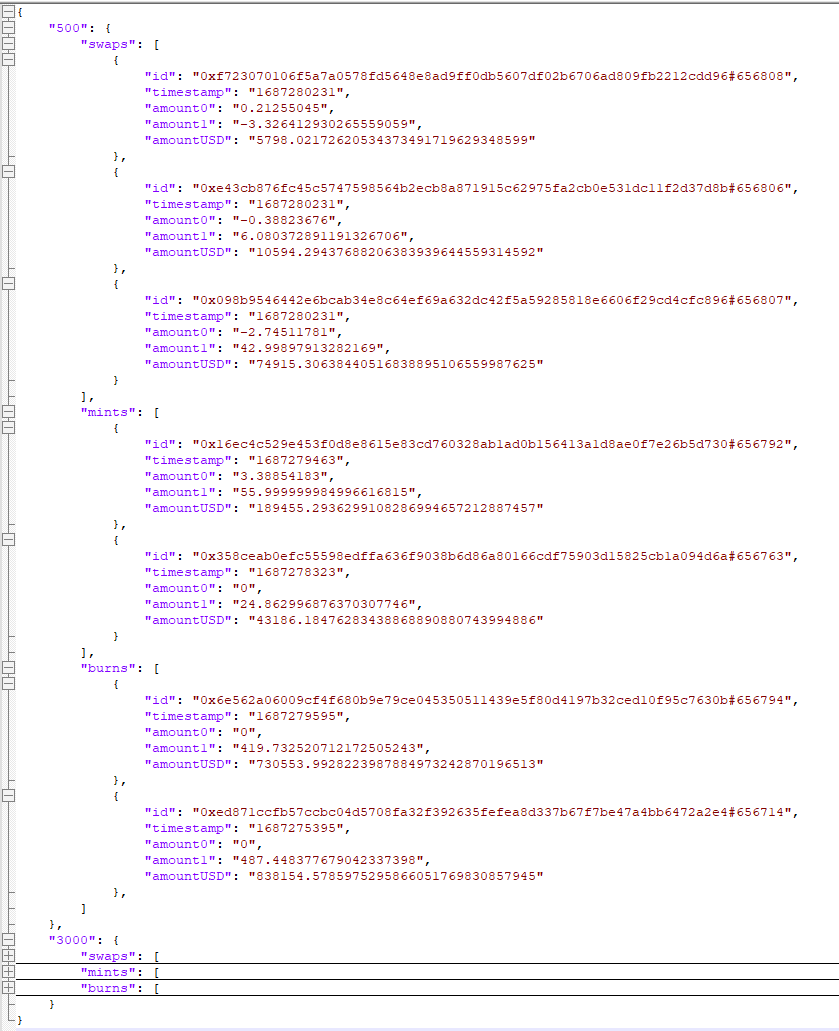
\includegraphics[width=\linewidth]{C:/Users/MatiasVizcaino/repos/Team-111/Other Resources/Data Screenshots - Uniswap.png}
\caption{Screenshot of Uniswap data.}
\label{fig:uniswap-screenshot}
\vspace{3pt} % Adjust the vertical spacing as needed
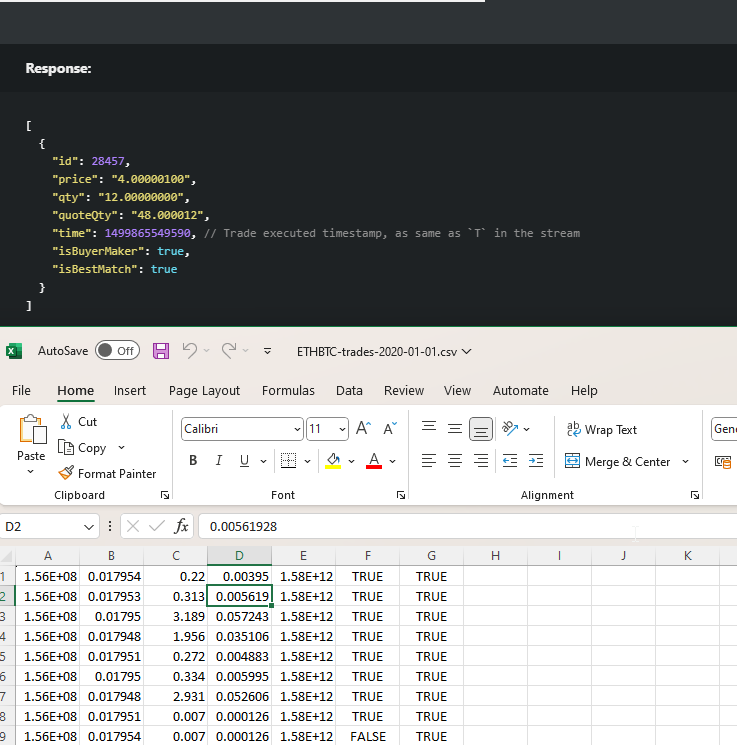
\includegraphics[width=\linewidth]{C:/Users/MatiasVizcaino/repos/Team-111/Other Resources/Data Screenshots - Binance.png}
\caption{Screenshot of Binance data.}
\label{fig:binance-screenshot}
\end{wrapfigure}

Inspired by the \textit{“DeFi modelling and forecasting trading volume" (2023)}\footnote{\textit{“DeFi: modeling and forecasting trading volume on Uniswap v3 liquidity pools"} (2023), \url{https://ssrn.com/abstract=444535}.} paper, we source and construct trade information for at least 6 months with the following sources:


\subsection*{1. Uniswap's The Graph API\footnote{Uniswap's The Graph API: \url{https://api.thegraph.com/subgraphs/name/uniswap/uniswap-v3}}}
\begin{minipage}[t]{0.78\textwidth}
Description: Provides transaction details, trading volumes, and block information from Uniswap v3 liquidity pools.
Focus: Specifically, we focus on the Uniswap v3 WBTC-WETH liquidity pools for fee tiers 400 and 3000. We would like to also add WBTC-USDC and USDC-WETH pools to consider Network spillover effects.
Available Attributes: Transaction IDs, timestamps, amounts, USD equivalents, and other related data.
\end{minipage}

\subsection*{2. Etherscan API\footnote{Etherscan API: \url{https://api.etherscan.io/api}} for Uniswap transaction hashes}
Description: Used to extract corresponding transaction data from Etherscan based on transaction hashes.
Data: Block hashes, block numbers, sender addresses, gas details, transaction hashes, and other relevant information.

\subsection*{3. Binance\footnote{Binance GitHub Repository: \url{https://github.com/binance/binance-public-data/blob/master/python/README.md}} CEX Data for ETHBTC}
\begin{minipage}[t]{0.78\textwidth}
Description: Daily zip trades downloaded using provided scripts from the Binance GitHub repository.
Data: Detailed information about each trade executed on the Binance platform, including trade prices, quantities, timestamps, and buyer/seller characteristics.
\end{minipage}

\section*{Key Variables}
\textbf{Independent Variable:} Liquidity pool trading volumes (amountUSD) over specific blocks.\\

\textbf{Dependent Variables:}
The dependent variables are derived from a set of features and can be categorized as follows:
\begin{enumerate}[label=\arabic*. ,itemsep=0pt, topsep=0pt]
\item Direct pool features: volatility, rate, number of trades, average trade size, total value locked (TVL).
\item Network spillover effects: trade flow imbalance.
\item CEX spillover effects: actual coin trade volume.
\item Price divergences between the 500 and 3000 pools.
\end{enumerate}

\section*{Approach}
\begin{enumerate}[itemsep=0pt, topsep=0pt]
\item Data Collection: Source data from multiple APIs (Uniswap, Binance) for liquidity pool sizes, trading volumes, and relevant variables. Associate data with Ethereum block numbers for consistent time measurement.
\item Data Preprocessing: Clean, format, and handle missing values. Ensure data consistency and address discrepancies arising from multiple sources.
\item Feature Engineering: Construct features to capture historical patterns, spillover effects, and price divergences. Utilize block-based time-series analysis framework.
\item Exploratory Data Analysis: Generate descriptive statistics, visualizations, and perform correlation analyses to uncover patterns, trends, and relationships between variables.
\item Model Selection and Development: Implement regression models (Linear Regression, Random Forest, Gradient Boosting) to investigate the pool size-trading volume relationship.
\item Model Evaluation and Optimization: Evaluate models using metrics (RMSE, MAE). Optimize selected model's hyperparameters using techniques like GridSearchCV or RandomizedSearchCV.
\item Final Analysis and Conclusions: Finalize analysis, draw conclusions, and communicate findings.
\end{enumerate}

Throughout this process, we aim to maintain rigorous documentation of our methodologies and findings, which will allow us to ensure the transparency and replicability of our research.

\section*{Anticipated Conclusions, Hypothesis, and Business Impact}

Through our analysis, we anticipate discovering a notable correlation between liquidity pool size and trading volume. Our hypothesis suggests that larger liquidity pools will demonstrate higher trading volumes, as they can facilitate larger transactions with minimal price impact.

The implications of our findings extend to various stakeholders within the ecosystem. For liquidity providers and traders, our research can provide insights to optimize their strategies, resulting in increased profits and minimized slippage. Additionally, DeFi platforms can leverage our analysis to design more efficient and appealing liquidity pools, fostering enhanced user engagement and driving overall platform growth.


\section*{Project Timeline}
\begin{description}[itemsep=0pt, topsep=0pt, leftmargin=1.5cm]
\item[Week 1] Data Collection and Cleaning
\begin{description}[itemsep=0pt, topsep=0pt, leftmargin=1cm]
\item[Task 1.1] Data extraction from APIs (Uniswap and Binance) and consolidating the data.
\item[Task 1.2] Initial data cleaning and preprocessing, which includes handling missing data and ensuring data consistency.
\end{description}
\item[Week 2] Feature Engineering and Exploratory Data Analysis
\begin{description}[itemsep=0pt, topsep=0pt, leftmargin=1cm]
\item[Task 2.1] Constructing new features based on the existing data and guided by previous research.
\item[Task 2.2] Conducting exploratory data analysis, generating descriptive statistics, and visualizations.
\end{description}
\item[Week 3] Model Selection and Initial Evaluation
\begin{description}[itemsep=0pt, topsep=0pt, leftmargin=1cm]
\item[Task 3.1] Implementing various regression models like Linear Regression, Random Forest, and Gradient Boosting to investigate the relationship between pool size and trading volume.
\item[Task 3.2] Conducting an initial evaluation of models based on metrics like RMSE and MAE.
\end{description}
\item[Week 4] Model Optimization and Final Evaluation
\begin{description}[itemsep=0pt, topsep=0pt, leftmargin=1cm]
\item[Task 4.1] Optimizing the hyperparameters of the selected model using techniques such as GridSearchCV or RandomizedSearchCV to improve their predictive performance.
\item[Task 4.2] Final evaluation of the models after hyperparameter optimization.
\end{description}
\item[Week 5] Results Interpretation, Report Writing, and Finalization
\begin{description}[itemsep=0pt, topsep=0pt, leftmargin=1cm]
\item[Task 5.1] Final analysis, interpreting the results, and drawing conclusions.
\item[Task 5.2] Writing and finalizing the report, which includes our findings and insights in relation to our initial research questions.
\item[Task 5.3] Reviewing and refining the report to ensure its quality and accuracy.
\end{description}
\end{description}

\end{document}
